\documentclass{ximera}

\title{Application Walkthrough 1: Mass of a Wire}
\author{Zack Reed}

\begin{document}
\begin{abstract}
This walkthrough will give you a good glimpse of some of the main ways we want to think about differentiating and integrating along curves when modeling phenomena using mathematics! This will also give you a rough template and introduce you to the tools that you can use for your mini project, due at the end of this module.
\end{abstract}
\maketitle

Just commenting everything out for now until the system resets and we can figure out why the html is not loading.

% \section*{Introduction}

% Welcome to your first project walkthrough!
% This walkthrough will give you a good glimpse of some of the main ways we want to think about differentiating and integrating along curves when modeling phenomena using mathematics! 

% This will also give you a rough template and introduce you to the tools that you can use for your mini project, due at the end of this module.

% \section*{Context: Mass of a Wire}

% We're going to look at various vector curves in space and imagine that they are skinny wires. The goal will be to calculate the mass of the wires using derivatives and integrals, but also to gut-check the mass of the wires with approximations.

% \subsection*{Basic Model: Mass = Density $\times$ Length}

% As with all things integral, you start with a basic model (typically involving multiplication) for quantifying something about a mathematical object. In this case, the basic model is:
% \[
% M = \rho \cdot L.
% \]
% Then, some variation in an object forces us to use integration instead of multiplication, adding up lots of small approximate pieces formed from the basic model.

% Many wires you come across are \emph{uniformly dense}. That is, no matter how big or small of a piece of wire, the ratio between the mass of the wire and the length of the wire will always be constant (i.e. a constant density).

% Let's take a look at a simple wire with constant density using the code found in the MATLAB script.

% \begin{expandable}{instructions}{MATLAB Instructions}
% \textit{The first line of code in the following cell sets up the variable, t.}

% \textit{The second line of code defines the wire curve as a vector function.}

% \textit{The third line enters the constant density.}

% \textit{The fourth line makes an animation showing the wire being broken up into smaller and smaller pieces but always having the same mass-length ratio between each piece.}

% \end{expandable}

% When you're ready, delete the percent sign in front of \texttt{animate\_segment\_cases(r,rho)} to show the animation in the following video.

% \begin{expandable}{code}{Show MATLAB Code}
% \texttt{syms t}\\
% \texttt{r=[sin(t), cos(t), t];}\\
% \texttt{rho=2}\\
% \texttt{animate\_segment\_cases(r,rho)}
% \end{expandable}

% We'll use the curve $\vec{r}(t) = [\sin(t), \cos(t), t]$ with constant density $\rho = 2$.

% % \begin{center}
% % \youtube{fKjpdnlIlIE}
% % \end{center}

% The animation shows the wire being broken up into smaller and smaller pieces but always having the same mass-length ratio between each piece.

% \subsection*{Checking Constant Mass}

% Use the slider to run through the animation after it finishes. You'll note that there is a constant ratio between the mass and the length no matter what the segment size is.

% \begin{problem}
% The density found from the total mass and total length is $\dfrac{17.772}{\answer[tolerance=.01]{8.886}} \approx \answer[tolerance=0.1]{2}$.  

% Now, for each displayed segment in the animation, you should find the masses and lengths of the smaller segments. Use these measures to verify that across these instances the wire density was indeed constant (within small numerical error).

% The length of the segment with a mass of $0.178$ is $\answer[tolerance=0.01]{0.089}$, making the density approximately $\answer[tolerance=0.1]{2}$.

% The mass of the segment with length $.178$ is $\answer[tolerance=0.01]{0.355}$, making the density approximately $\answer[tolerance=0.1]{2}$.

% \begin{feedback}
% Check the animation to get the mass-length pairs at the scales visualized.
% \end{feedback}

% The mass-to-length ratios for individual segments \wordChoice{\choice[correct]{agree}\choice{disagree}} with the overall density (up to rounding).
% \end{problem}

% \subsection*{Variable Density}

% Now see what happens if you have a variable density. We will set the density of the wire as the increasing function $\rho(t) = 2 + t^2$.

% Since $t$ is already defined as a variable in MATLAB, it does not need to be re-defined. We simply need to define a function that gives us the density along the wire.

% \begin{remark}
% To define the function in MATLAB, use the syntax \texttt{[function\_name]=[formula]}.

% \textit{Example:} \texttt{g=x\^{}2} defines the function $g(x)=x^2$.
% \end{remark}

% Now again use \texttt{animate\_segment\_cases}, using \texttt{r} as the first argument and then \texttt{rho} as the second argument.

% \begin{expandable}{instructions}{MATLAB Instructions}
% The function called ``rho'' is defined with the formula $2+t^2$.

% \texttt{rho=2+t\^{}2}\\
% \\
% \texttt{animate\_segment\_cases(r, rho)}
% \end{expandable}

% % \begin{center}
% % \youtube{FIFZBi8JPFU}
% % \end{center}

% The animation again uses \texttt{animate\_segment\_cases(r, rho)}, but now you should see that the mass changes as you move along the curve. This means that the density of this wire is not uniform.

% \subsection*{Variable Mass Along the Wire}

% You should see that the mass changes as you move along the curve. This means that the density of this wire is not uniform.

% The formula $\rho(t) = 2 + t^2$ should provide the density at any time $t$. 

% As before, slide through the animation and determine what the density is at $t=\pi$ and $t=2\pi$ (within the different scales in the animation). Verify (up to a little error) that $\rho$ determined the density at those times by dividing the mass by the length of the segments at those times.

% You can use the \texttt{subs()} command to verify the density values from $\rho$. 

% \begin{remark}
% \textit{Example:} Evaluating $\rho$ at time $t=2$ can be done using the command \texttt{subs(rho, t, 2)}, which means ``substitute into $\rho$, replacing the value $t$ with $2$.''
% \end{remark}

% \begin{expandable}{code}{Show MATLAB Code}
% \texttt{subs(rho,t,2)}\\
% \\
% \texttt{\% Now use subs() to verify the density values at time=pi and time=2*pi.}\\
% \texttt{\% Within a small error the density calculations from the animation and from}\\
% \texttt{\% the density function should agree.}
% \end{expandable}

% \begin{problem}
% If you need a gut-check, you can also just hand-calculate the density.

% Compute $\rho(\pi) = \answer[tolerance=0.01]{11.87}$ and $\rho(2\pi) = \answer[tolerance=0.01]{41.48}$ using either hand calculation or \texttt{subs}. 

% Within a small error, do the density calculations from the animation and from the density function agree? \wordChoice{\choice[correct]{Yes}\choice{No}}
% \end{problem}

% \section*{Challenges to the Basic Model: Variable Density}

% We want to calculate the mass of a wire just using multiplication, $M = \rho \cdot L$, where:
% \begin{itemize}
% \item $M$ is the mass of the wire,
% \item $\rho$ is the uniform density,
% \item $L$ is the length of the wire.
% \end{itemize}

% Unfortunately, we can't use this basic model for many wires because:
% \begin{itemize}
% \item Many wires have strange shapes and we don't want to stretch them out to measure their length.
% \item Not all wires have uniform densities, so there is no one density that will work in the basic model.
% \end{itemize}

% So, how do we compute the total length and total mass? We integrate to ``add up small mass pieces'' together.

% \section*{Step 1: Visualize the Approximate Pieces}

% Let's visualize the approximation process first. 

% The \texttt{plot\_curve\_pieces} course MATLAB function will:
% \begin{itemize}
% \item take in a wire as the first argument,
% \item a number of pieces ($N$) as the second argument,
% \item a density function as the third argument,
% \end{itemize}
% and will show you a plot of the wire pieces color-coded by density.

% \begin{remark}
% The plot called in the next cell is the example wire and density broken up into 20 pieces.
% \end{remark}

% \begin{expandable}{code}{Show MATLAB Code}
% \texttt{plot\_curve\_pieces(r,20,rho)}
% \end{expandable}

% You should see the wire broken up into 20 pieces, each piece having a slightly different color, noting the density of the midpoint of the piece (as an approximation for the density of the whole piece). (As exemplified in the following figure.)

% % \begin{center}
% % 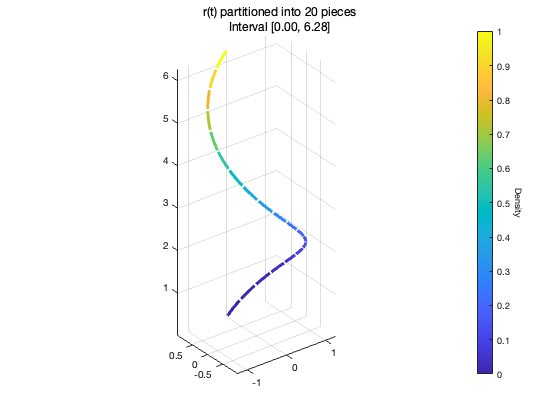
\includegraphics[width=0.5\textwidth]{20_seg_wire.png}
% % \end{center}

% This effectively sets up a \emph{midpoint approximation} of the mass. That is, the density at the midpoint of the segment is treated as the uniform density of the entire segment.

% \subsection*{Midpoint Mass Plot}

% The function \texttt{plot\_curve\_mass\_pieces} will also use the same arguments (\texttt{r}, \texttt{N}, \texttt{rho}) but the plot will tell you the mass approximated by the midpoint sum in the title.

% \begin{expandable}{code}{Show MATLAB Code}
% \texttt{N=20}\\
% \texttt{plot\_curve\_mass\_pieces(r,N,rho)}
% \end{expandable}

% \begin{problem}
% If everything is set up correctly, what approximate mass is reported by the 20-piece midpoint plot? 

% A 20-piece sample midpoint approximation of the mass should measure $\answer[tolerance=0.01]{134.354}$ grams.

%     \begin{feedback}
%     You should see the following figure with the mass in the title.
%         % \begin{center}
%         % 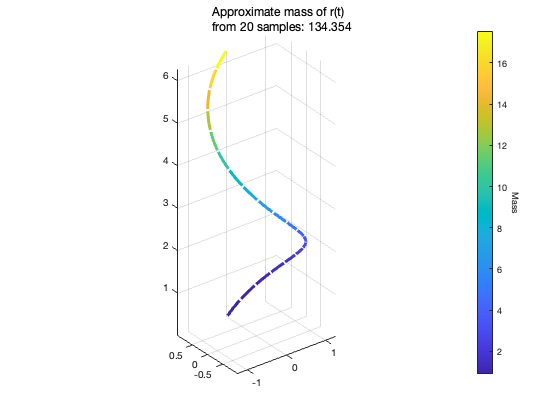
\includegraphics[width=0.5\textwidth]{20_mass_approx.png}
%         % \end{center}
%     \end{feedback}
% \end{problem}

% \section*{Step 2: Approximate the Wire Mass}

% Let's make this approximation ourselves!

% Remember that mass is approximated by the product $M = \rho \cdot L$, ``density times the length''.

% So, if we had the lengths and densities of our wire after breaking it up into $N$ pieces, we could just multiply those densities and lengths to get the mass of each individual piece.

% This is exactly what the course function \texttt{break\_into\_pieces()} does!

% \begin{remark}
% If you've defined \texttt{r}, \texttt{N}, and \texttt{rho}, the following cell should give you lists (called arrays) of the densities at the midpoints of the N wire segments as well as the segment lengths, called ``densities'' and ``lengths''.
% \end{remark}

% \begin{expandable}{code}{Show MATLAB Code}
% \texttt{[\textasciitilde, lengths, densities, \textasciitilde, \textasciitilde] = break\_into\_pieces(r, N, rho)}
% \end{expandable}

% In your output, you should see two $1\times20$ lists (called arrays), ``lengths'' and ``densities''. The numbers in each are the lengths of the broken wire and the densities of the broken wire.

% \subsection*{20-Piece Approximation of Mass}

% Now we're going to use \texttt{lengths} and \texttt{densities} to do some quick approximations.

% One really nice feature of MATLAB is that it can do many many calculations at once! For instance, ``\texttt{.*}'' will multiply the entries of two arrays at matching index values.

% \begin{remark}
% Remember that the index, $i$ of a list or of a sum, is just the number telling how far in the list (or sum) to look. So the 2nd element of ``densities'' is the second number in the densities list, the 4th element of ``lengths'' is the fourth number in the list, etc.
% \end{remark}

% \begin{expandable}{instructions}{MATLAB Instructions}
% The following cell uses \texttt{.*} to multiply each entry in densities by the same entry in lengths. This will quickly multiply all of the approximate densities by the approximate lengths.
% \end{expandable}

% \begin{expandable}{code}{Show MATLAB Code}
% \texttt{masses=densities.*lengths}
% \end{expandable}

% You should see a 20-length list of masses whose entries are the products of the corresponding entries in \texttt{lengths} and \texttt{densities}.

% \begin{expandable}{instructions}{MATLAB Instructions}
% The next cell uses \texttt{sum()} to add the entries in ``masses'' to find the approximate mass of the 20-piece wire.
% \end{expandable}

% \begin{expandable}{code}{Show MATLAB Code}
% \texttt{mass\_approx=sum(masses)}
% \end{expandable}

% The result of the sum should closely match the approximation from the plot!

%     % \begin{center}
%     % 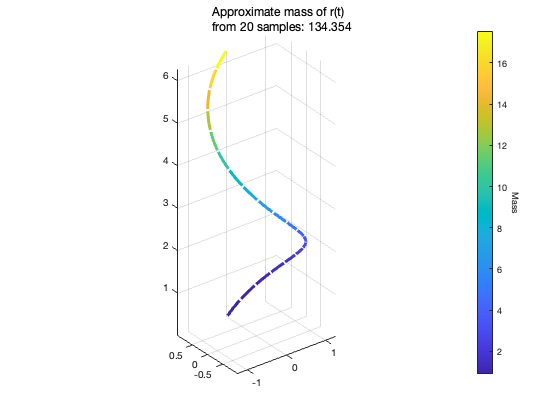
\includegraphics[width=0.5\textwidth]{20_mass_approx.png}
%     % \end{center}

% \begin{problem}
% Record the first three entries from your \texttt{lengths} array: $\answer[tolerance=0.01]{1.01}$, $\answer[tolerance=0.01]{1.01}$, $\answer[tolerance=0.01]{1.01}$

% Record the first three entries from your \texttt{densities} array: $\answer[tolerance=0.1]{2.25}$, $\answer[tolerance=0.1]{3.23}$, $\answer[tolerance=0.1]{4.21}$

% Compute \texttt{mass\_approx} for $N=20$: $\answer[tolerance=0.01]{134.354}$

% Does this match the value from \texttt{plot\_curve\_mass\_pieces}? \wordChoice{\choice[correct]{Yes}\choice{No}}
% \end{problem}

% \subsection*{Symbolizing: Midpoint Sum Approximation}

% Hopefully you see the same number in \texttt{mass\_approx} and in the figure!

% As you've seen in previous courses, especially with Riemann Sums, to symbolically write out our approximation:
% \begin{itemize}
% \item We call $M$ the approximate mass and $\Delta M$ the individual small masses,
% \item Our approximation was simply $M \approx \sum_i \Delta M_i$ ``$M$ is approximately the sum of the small masses''.
% \end{itemize}

% In this case, we measured the masses using the density$\times$length products. So:
% \begin{itemize}
% \item Each $\Delta M_i = \rho_i \Delta L_i$, the product of the density and the changes in length,
% \item The new approximation becomes $M \approx \sum_i \Delta M_i = \sum_i \rho_i \Delta L_i$.
% \end{itemize}

% Notice that we found all of the masses from the product \texttt{masses = densities .* lengths} and then summed the list of products, so the symbols match our approximation process!

% \section*{Refining the Approximation Using Smaller Scales}

% This approximation works at any scale, and by now we're familiar with the basic principle of approximations getting better as we get on smaller scales (increasing $N$).

% The following code re-creates the approximation for a few different values of $N$, making more refined approximations each time.

% \begin{remark}
% At the end of each line except for \texttt{mass\_approx}, there is a semi-colon ``\texttt{;}''. This hides the output in your live script so that you're not overwhelmed by lots of calculations at once. This is a common trick when making many calculations.

% The plots may take a while to generate.

% If you want, you can do this in a for-loop instead, but you don't have to if you're unfamiliar with loops.
% \end{remark}

% \begin{expandable}{code}{Show MATLAB Code}
% \texttt{N = 50}\\
% \texttt{[\textasciitilde, lengths, densities, \textasciitilde, \textasciitilde] = break\_into\_pieces(r, N, rho);}\\
% \texttt{masses = densities .* lengths;}\\
% \texttt{mass\_approx = sum(masses)}\\
% \texttt{plot\_curve\_mass\_pieces(r, N, rho);}\\
% \\
% \texttt{N = 100}\\
% \texttt{[\textasciitilde, lengths, densities, \textasciitilde, \textasciitilde] = break\_into\_pieces(r, N, rho);}\\
% \texttt{masses = densities .* lengths;}\\
% \texttt{mass\_approx = sum(masses)}\\
% \texttt{plot\_curve\_mass\_pieces(r, N, rho);}\\
% \\
% \texttt{N = 150}\\
% \texttt{[\textasciitilde, lengths, densities, \textasciitilde, \textasciitilde] = break\_into\_pieces(r, N, rho);}\\
% \texttt{masses = densities .* lengths;}\\
% \texttt{mass\_approx = sum(masses)}\\
% \texttt{plot\_curve\_mass\_pieces(r, N, rho);}
% \end{expandable}

% \begin{problem}
% Record \texttt{mass\_approx} for $N=50$: $\answer[tolerance=0.01]{134.648}$

% Record \texttt{mass\_approx} for $N=100$: $\answer[tolerance=0.01]{134.690}$

% Record \texttt{mass\_approx} for $N=150$: $\answer[tolerance=0.01]{134.697}$

% What trend do you observe? \begin{multipleChoice}
% \choice[correct]{The approximations are increasing and converging to a value}
% \choice{The approximations are decreasing}
% \choice{The approximations are oscillating}
% \choice{No clear trend}
% \end{multipleChoice}

% \begin{feedback}
%     The following plots should appear for each $N$ value.
%         % \begin{center}
%         % 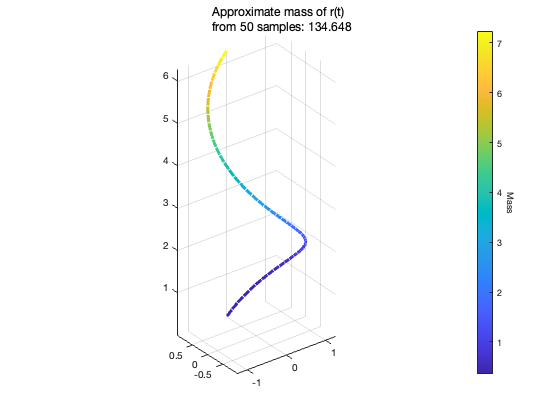
\includegraphics[width=0.5\textwidth]{50_mass_approx.png}
%         % 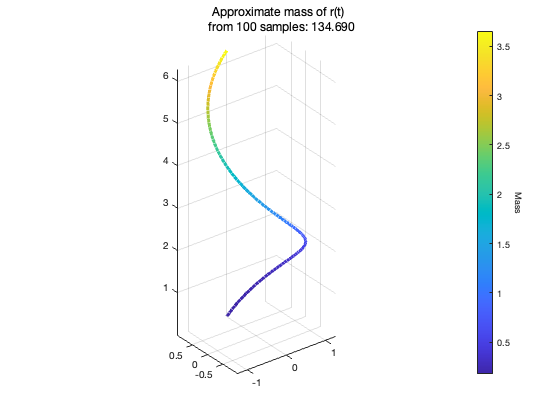
\includegraphics[width=0.5\textwidth]{100_mass_approx.png}
%         % 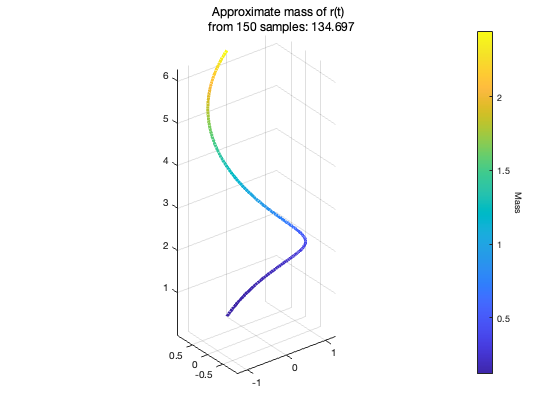
\includegraphics[width=0.5\textwidth]{150_mass_approx.png}
%         % \end{center}
% \end{feedback}
% \end{problem}

% \subsection*{Very Small Scales}

% Now we do the calculations again but for larger values of $N$. This will get the approximation within the standard double precision in MATLAB.

% \begin{expandable}{code}{Show MATLAB Code}
% \texttt{N = 1000}\\
% \texttt{[\textasciitilde, lengths, densities, \textasciitilde, \textasciitilde] = break\_into\_pieces(r, N, rho);}\\
% \texttt{masses = densities .* lengths;}\\
% \texttt{mass\_approx = sum(masses)}\\
% \\
% \texttt{N = 10000}\\
% \texttt{[\textasciitilde, lengths, densities, \textasciitilde, \textasciitilde] = break\_into\_pieces(r, N, rho);}\\
% \texttt{masses = densities .* lengths;}\\
% \texttt{mass\_approx = sum(masses)}\\
% \\
% \texttt{N = 100000}\\
% \texttt{[\textasciitilde, lengths, densities, \textasciitilde, \textasciitilde] = break\_into\_pieces(r, N, rho);}\\
% \texttt{masses = densities .* lengths;}\\
% \texttt{mass\_approx = sum(masses)}
% \end{expandable}

% \begin{problem}
% Record the three large-$N$ approximations:

% For $N=1000$: $\answer[tolerance=0.01]{136.11}$

% For $N=10000$: $\answer[tolerance=0.001]{136.127}$

% For $N=100000$: $\answer[tolerance=0.001]{136.127}$

% Notice that the last two $N$-values gave the same approximation. This does not mean we found the exact mass, it simply means we surpassed the default precision of MATLAB.

% If the last two agree to machine precision, what does that suggest? \begin{multipleChoice}
% \choice[correct]{We have found a very accurate approximation}
% \choice{We have found the exact value}
% \choice{The approximation method is failing}
% \choice{We need to increase $N$ further}
% \end{multipleChoice}
% \end{problem}

% \section*{Generating Exact Measures: Integration}

% Let's see if we can use integrals to get a more exact measure, and double check that it's close to our approximations!

% The key with integrating is that we're still adding up small bits of mass to get an exact measure of mass. The ``small bits'' we're integrating are differential bits whose total sum represent the limit of the finite sums.

% \subsection*{Symbolizing}

% Let's translate our finite approximations into integrals to get an idea of how we want to set up the integral for computation.

% \begin{itemize}
% \item The approximation equation $M \approx \sum \Delta M$ becomes $M = \int dM$, ``add up tiny bits of mass to get the total mass''.
% \item The small bit of mass comes from the density$\times$length products on a small bit of arc length along the curve, $dL$, so our equation for mass becomes $M = \int dM = \int \rho \, dL$. ``The total mass comes from adding up small density$\times$length products along the wire''.
% \end{itemize}

% \subsection*{New Need: Using the Fundamental Theorem of Calculus}

% The main trick when computing integrals is using the Fundamental Theorem of Calculus (FTC):

% The FTC is useable for differential products of the form $dF = f \cdot dt$ so that we can make use of antiderivatives to find explicit formulas for $F$.

% Since the curve and density are defined by time, without doing some kind of substitution we can't immediately use the FTC when we integrate with respect to Mass or Length.

% Luckily, we know how to differentially represent the arc length differential from a curve's velocity magnitude!
% \[
% dL = \|\vec{v}\| \cdot dt
% \]

% So, with one final re-write of our equations, we get
% \[
% M = \int dM = \int \rho \, dL = \int_a^b \rho(t) \|\vec{v}(t)\| \, dt
% \]
% and we have a representation of our sum with which we can use the FTC!

% \subsection*{Building and Computing the Integral}

% We can use \texttt{diff()} and \texttt{norm()} to find the velocity of our curve, and then use \texttt{int()} plugging in all the values to get an integral of the exact mass!

% First, we get the velocity of the curve using \texttt{diff()}:

% \begin{expandable}{code}{Show MATLAB Code}
% \texttt{v=diff(r)}
% \end{expandable}

% You should see a vector representing the derivatives of the coordinate functions for $\vec{r}$.

% Now we use \texttt{norm()} to take the magnitude of the velocity function:

% \begin{expandable}{code}{Show MATLAB Code}
% \texttt{v\_mag=norm(v)}
% \end{expandable}

% The differential $dM = \rho \cdot dL = \rho \cdot \|\vec{v}\| \cdot dt$, so we enter the differential in MATLAB.

% \begin{remark}
% We don't put $dt$ into MATLAB, it is incorporated already when we use \texttt{int()}.
% \end{remark}

% \begin{expandable}{code}{Show MATLAB Code}
% \texttt{dM=rho*v\_mag}
% \end{expandable}

% Now we're ready to integrate!

% \texttt{int()} takes in:
% \begin{itemize}
% \item the function to be integrated
% \item the starting value for integrating (i.e. the ``$a$'' value)
% \item the ending value for integration (i.e. the ``$b$'' value)
% \end{itemize}

% It will then give you either:
% \begin{itemize}
% \item the number computed by the definite integral
% \item or a re-writing of the integral if the computer can't find a nice number
% \end{itemize}

% \begin{expandable}{code}{Show MATLAB Code}
% \texttt{M=int(dM,0,2*pi)}
% \end{expandable}

% \subsection*{Checking Our Results!}

% Likely, \texttt{M} didn't give you an exact number, it just wrote out the integral and the formula is a bit unwieldy.

% That's okay! Many functions don't have nice integrals (and often it's impossible to find antiderivatives).

% We can get a numerical approximation of the value using \texttt{double()}:

% \begin{expandable}{code}{Show MATLAB Code}
% \texttt{int\_approx=double(M)}
% \end{expandable}

% \begin{problem}
% Report the numerical value from \texttt{double(M)}: $\answer[tolerance=0.001]{136.127}$

% How does it compare with your high-$N$ approximations? \begin{multipleChoice}
% \choice[correct]{They agree within small numerical error}
% \choice{They differ significantly}
% \choice{The integral value is much larger}
% \choice{The integral value is much smaller}
% \end{multipleChoice}

% Hopefully, you get the same approximation (or very close) as we did with our high-$N$ approximations!
% \end{problem}

% \section*{Your Turn: Use Your Own Curve}

% Now you try! Go through the steps yourself, for your own curve, which will mirror the same steps you'll need to take for the mini project.

% Define your curve $\vec{r}$ that you will use in the Module 3 mini project, then define the density to be the $\rho$ function you were provided (the wire density or the air density depending on your application) and then select a number of pieces (not too big) to break up your wire.

% \begin{expandable}{instructions}{MATLAB Instructions}
% \textit{Define your vector curve using} \texttt{r = [x(t), y(t), z(t)]}\textit{, filling in the blanks.}

% \textit{Define your density using} \texttt{rho = \_\_\_\_}\textit{, filling in the blank with the formula for your ``density''.}

% \textit{Define the number of pieces you want to see, like} \texttt{N=50}.

% \textit{View the broken wire using} \texttt{plot\_curve\_pieces(r,N,rho)}.
% \end{expandable}

% \begin{expandable}{code}{Show MATLAB Code}
% \texttt{\% Define your vector curve using r = [x(t), y(t), z(t)]}\\
% \texttt{\% r = [\; ...\; , \; ...\; , \; ...\; ];}\\
% \\
% \texttt{\% Define your density using rho = \_\_\_\_}\\
% \texttt{\% rho = ...;}\\
% \\
% \texttt{\% Define the number of pieces you want to see}\\
% \texttt{\% N = 50;}\\
% \\
% \texttt{\% View the broken wire}\\
% \texttt{\% plot\_curve\_pieces(r, N, rho)}
% \end{expandable}

% Now manually compute the approximation:

% \begin{expandable}{instructions}{MATLAB Instructions}
% \textit{Recreate the mass approximations using} \texttt{break\_into\_pieces} \textit{and the steps earlier in the script.}

% \textit{Do so at a few scales and check that the approximations agree with the prompts.}

% \textit{Well-approximate the mass of your curve with high-N calculations.}
% \end{expandable}

% \begin{expandable}{code}{Show MATLAB Code}
% \texttt{\% Recreate the mass approximations using break\_into\_pieces}\\
% \texttt{\% [\textasciitilde, lengths, densities, \textasciitilde, \textasciitilde] = break\_into\_pieces(r, N, rho);}\\
% \texttt{\% masses = densities .* lengths;}\\
% \texttt{\% mass\_approx = sum(masses);}\\
% \\
% \texttt{\% Do so at a few scales and check that the approximations agree}\\
% \\
% \texttt{\% Well-approximate the mass of your curve with high-N calculations}
% \end{expandable}

% Now use integrals to verify your measures:

% \begin{expandable}{instructions}{MATLAB Instructions}
% \textit{Use} \texttt{diff()}\textit{,} \texttt{norm()} \textit{and} \texttt{int()} \textit{to generate the integral measure of the mass.}

% \textit{Use a} \texttt{double()} \textit{approximation to compare with your midpoint approximations.}
% \end{expandable}

% \begin{expandable}{code}{Show MATLAB Code}
% \texttt{\% Use diff(), norm() and int() to generate the integral measure}\\
% \texttt{\% v = diff(r);}\\
% \texttt{\% v\_mag = norm(v);}\\
% \texttt{\% dM = rho * v\_mag;}\\
% \texttt{\% M = int(dM, a, b);}\\
% \\
% \texttt{\% Use double() to compare with your midpoint approximations}\\
% \texttt{\% int\_approx = double(M)}
% \end{expandable}

% \begin{problem}
% Record your final midpoint approximation (for some large $N$): $\answer[tolerance=1]{0}$

% Record your integral approximation: $\answer[tolerance=1]{0}$

% Do they agree within a reasonable tolerance? \wordChoice{\choice{Yes}\choice{No}\choice{Not yet tested}}
% \end{problem}

% \section*{Conclusion}

% We've just gone through the similar steps that you'll go through in detail for your projects, but this attention to arc length will give you a head start on your projects, as those integrals will build on the arc length and mass integrals.

% You have:
% \begin{itemize}
% \item Used midpoint approximations to estimate mass as a sum of $\rho \cdot \Delta L$,
% \item Refined the approximation by increasing $N$,
% \item Derived and computed the exact integral $M = \int_a^b \rho(t) \|\vec{r}'(t)\| \, dt$,
% \item Compared numerical and exact approaches for validation.
% \end{itemize}



\end{document}